\chapter{Recuperación de imágenes basadas en su contenido (CBIR)}

En el contexto de las ciencias de información, en el Capítulo 1 de \cite{10.5555/1394399} podemos encontrar una definición genérica para el contexto de las ciencias de computación del término "recuperación de información" que dice que:

\begin{definicion}
La recuperación de información, o \emph{information retrieval (IR)}, consiste en encontrar material de una naturaleza no estructurada que satisface una necesidad de información dentro de grandes colecciones.
\end{definicion}

En particular, nos encontramos trabajando en la recuperación de imágenes que pertenece a la categoría de recuperación de información multimedia. Este, a su vez, se divide en dos tipos de recuperación, las basadas en texto, \emph{text-based image retrieval (TBIR)}, o las basadas en su contenido, \emph{content-based image retrieval (CBIR)}.\\

En \cite{content-based} se dice, en que los sistemas TBIR, los usuarios utilizan palabras clave o descripciones de las imágenes como consulta en una base de datos para recuperar las imágenes que sean relevantes a la palabra clave. Para ello, primeramente las imágenes deben de ser anotados con texto ya sea de forma manual o automática. Esto posee la desventaja de que los algoritmos de anotación automática de imágenes no son factibles para generar textos descriptivos para un amplio espectro de imágenes requiriendo la anotación manual que, a su vez, suele ser subjetiva y dependiente del contexto. Como ventaja, al realizar utilizar únicamente texto para describir la imagen, sus consultas son rápidas ya que la coincidencia de cadenas es un proceso que requiere menos tiempo de cómputo.\\

Por otro lado, la recuperación de imágenes basada en el contenido (CBIR), también conocida como consulta por el contenido de una imagen o \emph{query by image content (QBIC)}, es una técnica automatizada que toma una imagen como consulta y devuelve un conjunto de imágenes similares a esta \cite{content-based}. La imagen consultada es convertida en la representación interna de un vector de características usando la misma rutina de extracción que fue utilizada para crear la base de datos. Se utiliza una medida de similitud para calcular las distancias entre los vectores de características de la imagen consultada y de las imágenes destino en la base de datos de características. Por último, la recuperación se realiza mediante un esquema de indexación que facilita la búsqueda eficiente de la base de datos de imágenes \autoref{fig:content-based-esquema}.\\

\begin{figure}[htpb]
  \centering
  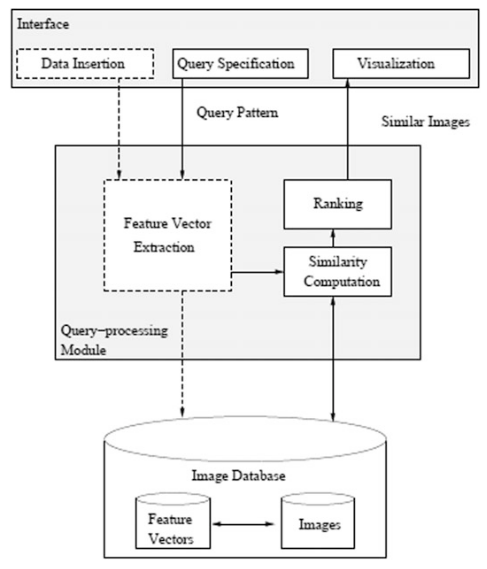
\includegraphics[width=0.55\textwidth]{content-based-esquema}
  \caption{Arquitectura de un sistema CBIR típico. \cite{content-based}}
  \label{fig:content-based-esquema}
\end{figure}

En las páginas 7-8 y 22-26 de \cite{report:39} se mencionan tres niveles de consultas en un CBIR siendo:

\begin{itemize}
\item Nivel 1: La recuperación de imágenes a través de características primitivas como pueden ser diferentes medidas de representación matemática de colores, texturas o formas. Un ejemplo sería un histograma de color que muestra la proporción de píxeles de cada color dentro de la imagen y la consulta sería encontrar imágenes con valores similares.
\item Nivel 2: Comprende la recuperación por características derivadas, también conocidas como lógicas, incluyendo un cierto grado de inferencia lógica sobre la identidad de los objetos representados en la imagen. Además puede ser dividido en:
\begin{itemize}
\item recuperación de objetos de un determinado tipo o categoría. Por ejemplo, ``encuentra imágenes de un autobús de dos pisos''.
\item recuperación de objetos individuales o personas. Por ejemplo, ``encuentra una imagen de la torre Eiffle''.
\end{itemize}
\item Nivel 3: Se trata de la recuperación por atributos abstractos, incluyendo una cantidad significativa de razonamiento de alto nivel sobre el propósito de los objetos o escenas representadas. Por ejemplo, ``encuentra imágenes de una multitud alegre''.
\end{itemize}

El objetivo de este proyecto es desarrollar una aplicación en java que represente un sistema CBIR que siga una arquitectura como la mostrada en \autoref{fig:content-based-esquema}. Este será capaz de extraer distintas características de una imagen y de comparar, o calcular la similitud, entre las imágenes de distintas formas para obtener distintas clasificaciones ordenadas que serán visualizadas en la aplicación. \\

Se podrán realizar consultas de nivel 1 a través de características de color y de nivel 2 utilizando segmentación semántica para la distinción de categorías con una red neuronal implementada en Python.

\chapter{Planificación y presupuesto.}
\chapter{Requisitos}
Antes de desarrollar la aplicación se debe comenzar con la exposición de los requisitos de datos, funcionales y no funcionales que esta requerirá para así poder tener en mente qué es lo que necesitamos, de qué es lo disponemos y cómo podremos trabajar de forma óptima para llegar al resultado deseado.\\

Teniendo en mente \autoref{fig:content-based-esquema}, sabemos que debemos de tener los siguientes requisitos de datos:\\
\begin{enumerate}
\item Representación de una imagen
\item Vector de características, en adelante descriptor, por cada característica que se quiera extraer o analizar.
\item Base de datos capaz de almacenar los descriptores correspondientes a cada una de las imágenes que estarán almacenadas en dicha base o fácilmente accesibles a través de la información almacenada en ella.
\item Representación de un descriptor genérico almacenado en la base de datos.
\item Concepto de clasificador utilizado para extraer las características.
\item Concepto de comparador para calcular la similitud entre las distintas características.
\end{enumerate}
Seguidamente, respecto a los requisitos funcionales debemos de considerar:\\
\begin{enumerate}
\item Abrir, guardar y cerrar una imagen.
\item Realización de consultas basadas en el contenido de una imagen.
\item Realización de consultas basadas en texto, siendo estas las categorías a las cuales pueden pertenecer nuestras imágenes.
\item Agrupación de categorías.
\item Extracción de descriptores de nivel 1.
\item Extracción de un descriptor de nivel 2.
\item Almacenaje de un conjunto de imágenes para poder ser comparadas.
\item Crer, modificar, guardar y abrir bases de datos.
\item Almacenaje de los descriptores correspondientes a dichas imágenes en una base de datos.
\item Enlace entre las imágenes y sus correspondientes descriptores para un fácil acceso.
\item Comparación entre descriptores.
\item Comparación utilizando múltiples descriptores de las propias imágenes.
\item Ordenación de imágenes resultantes de la consulta utilizando el resultado de la comparación entre descriptores.
\item Capacidad de visualizar las imágenes resultado de forma ordenada según la puntuación obtenida.
\item Capacidad de cambiar los comparadores utilizados sin que se vean afectados los descriptores utilizados.
\item Capacidad de crear nuevas bases de datos utilizando diferentes descriptores.
\item Capacidad de crear nuevas bases de datos utilizando múltiples descriptores.
\item Importar un clasificador a través de un fichero.
\end{enumerate}
Por último, respecto a los requisitos no funcionales nos referimos a las características de funcionamiento que nos servirán para mantener la calidad de nuestro programa. Estos serán, principalmente: rendimiento, durabilidad, estabilidad, seguridad, eficiencia, compatibilidad, garantía e integración de datos.

\chapter{Análisis}

\chapter{Diseño}
